\subsection{Opret Bruger}\label{sec:Opretbruger}
Dette afsnit indeholder en gennemgang af den grafisk brugergrænseflade, design og implementering af 'Opret Bruger' viewet i Rambøll Tilsyn.

\subsubsection{Design}
På Figur \ref{fig:OpretBrugerSekvens} ses sekvensdiagrammet for 'Opret bruger' viewet til Rambøll Tilsyn.
\begin{figure}[H] % (alternativt [H])
	\centering
	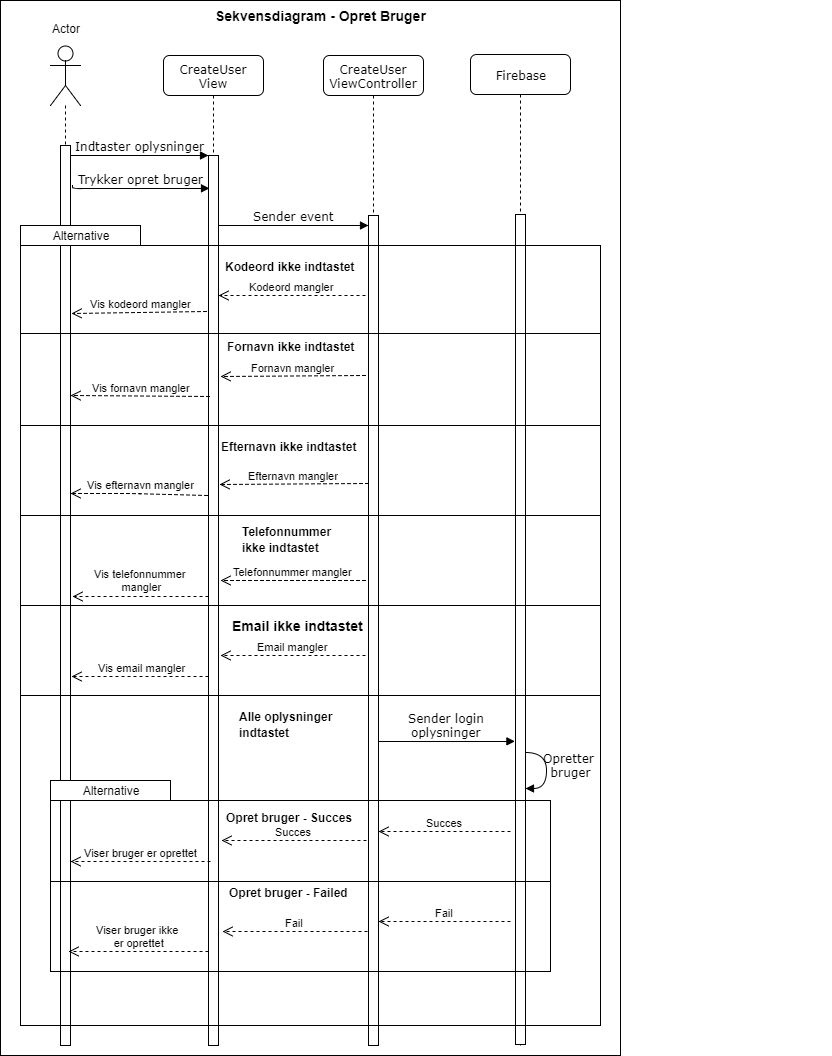
\includegraphics[height=20cm, width=15cm]{../ArkitekturDesign/Design/OpretBruger/OpretBrugerSekvensDiagram}
	\caption{Sekvensdiagram for 'Opret bruger' i Rambøll Tilsyn.}
	\label{fig:OpretBrugerSekvens}
\end{figure}

\subsubsection{Grafisk brugergrænseflade}
I OpretBrugerViewet er der lavet felter til alt det information, som skal tastes ind om en bruger. Se Figur \ref{fig:OpretBrugerView}
\begin{figure}[H] % (alternativt [H])
	\centering
	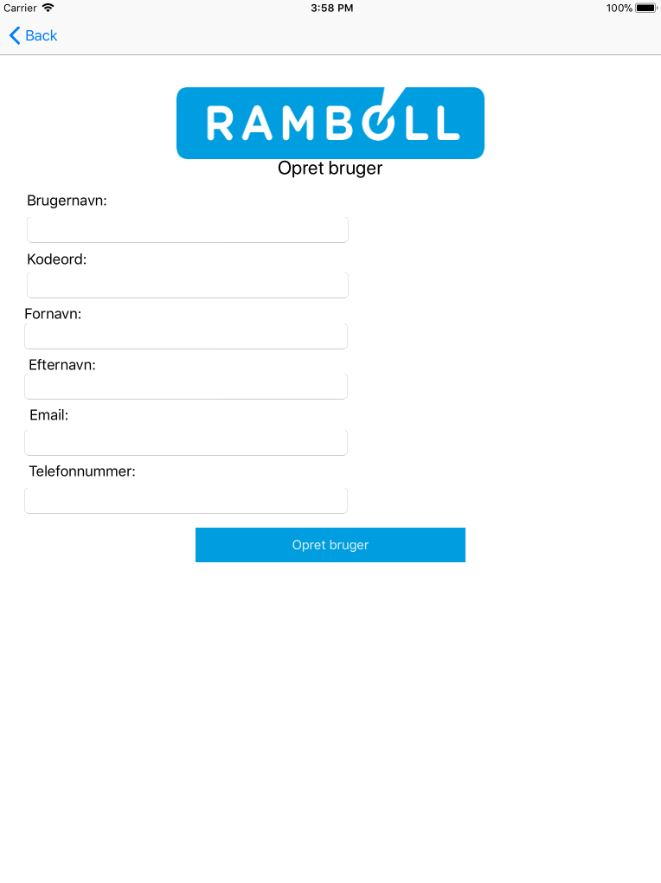
\includegraphics[height=12cm, width=10cm]{../ArkitekturDesign/Design/OpretBruger/OpretBrugerView}
	\caption{'Opret bruger' viewet som det er implementeret i Rambøll Tilsyn.}
	\label{fig:OpretBrugerView}
\end{figure}

\clearpage

\subsubsection{Implementering}
I dette afsnit vil der blive beskrevet funktionaliteten for de vigtigste funktioner i koden tilhørende 'Opret bruger' viewet.

På Figur \ref{fig:CreateUser}, ses funktionen for CreateUser().
\begin{figure}[H] % (alternativt [H])
	\centering
	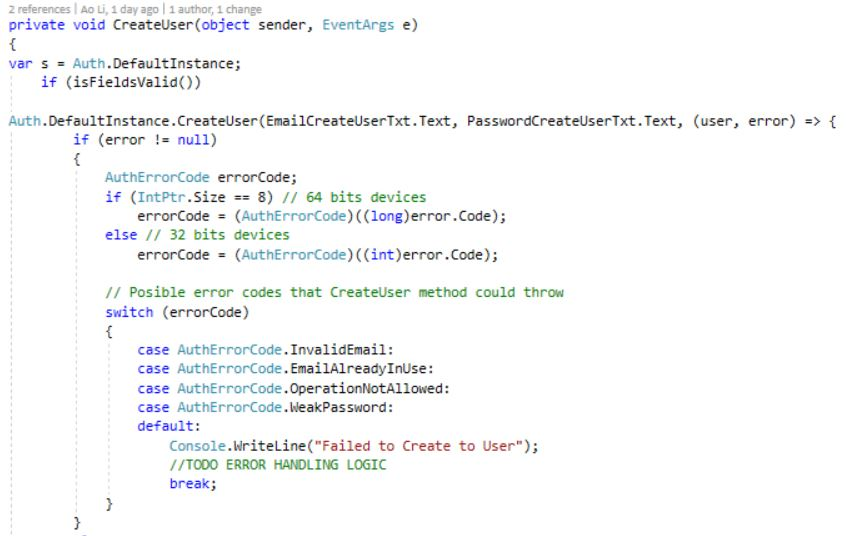
\includegraphics[height=8cm, width=17cm]{../ArkitekturDesign/Design/OpretBruger/CreateUser1}
\end{figure}
\begin{figure}[H] % (alternativt [H])
	\centering
	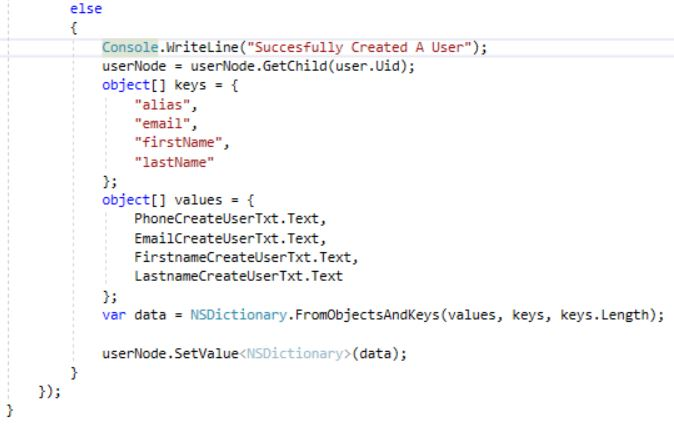
\includegraphics[height=8cm, width=17cm]{../ArkitekturDesign/Design/OpretBruger/CreateUser2}
	\caption{Kode snip - CreateUser() fra CreateUser.cs}
	\label{fig:CreateUser}
\end{figure}
Alle felter valideres. Derefter, hvis alt er godkendt, oprettes brugeren med de input, der er kommet fra viewet. Når brugeren er blevet oprettet uden problemer, skrives informationen som ikke har noget med log ind at gøre; Fornavn, Efternavn osv. ind i databasen.

\clearpage